\chapter{Key management systems}

With an increasing number of encryption keys to store and protect, there might be necessary to consider using key management server.
Key management server should provide a secure and persistent service to its clients providing:
\begin{itemize}
    \item key generation
    \item key exchange
    \item key storage,
    \item use
    \item crypto-shredding
    \item key replacement
\end{itemize}
One of the possible solutions for persistent key management is to deploy a key escrow server.

With key escrow a third party gets copies of a cryptographic key.
This third party, for example law enforcement, has the ability to decrypt encrypted data using our keys in escrow if they had the right.
People might not be comfortable with any third party, especially the government, having this ability and that "technical" problems vex the key escrow solution.

Key recovery, on the other hand, lets us just backup and restore cryptographic keys without any third party possesing our key.

Key recovery is necessary.
Key escrow is not.
Let us not confuse these two.

\section{Key Escrow server}\label{escrow}

Key Escrow server (also known as a “fair” cryptosystem) is a server providing escrow service for encryption keys.
A client using Key Escrow usually generates a key, encrypts data with it and then stores the key encryption key on a remote server.
However, it is not as simple as it sounds and there are couple of security concerns.

To deliver these keys we want to store on Escrow server, we have to encrypt the channel on which we distribute them.
When transmitting keys over non secure network without encrypted link, anyone listening to the network traffic could immadiately fetch the key.
This should signal security risks, and, of course, we do not want any third party to access our secret data.
Usually we encrypt a channel with TLS(Transport Layer Security) or GSSAPI (Generic Security Services Application Program Interface) as shown on a Figure \ref{fig:escrowmodel} Escrow model.
\begin{figure}[h]
    \centering
    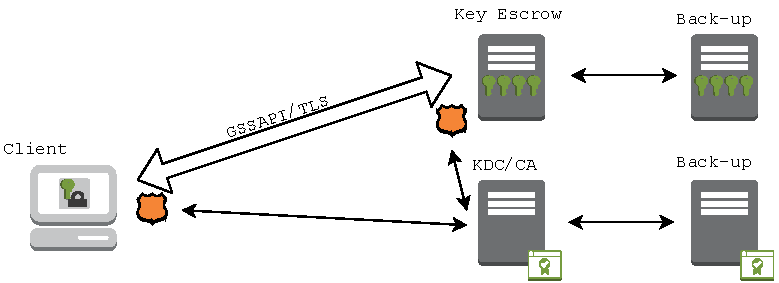
\includegraphics[scale=0.7]{figures/EscrowModel.pdf}
    \caption{Escrow model}
    \label{fig:escrowmodel}
\end{figure}
Unfortunatelly, this is not enough to have the communication secure.
We can not just start sending these keys to the escrow server, if we do not know whether this server is the one it acts to be.
This server has to have its own identity to be verified, and the client have to authenticate to this server too.
Increasing amount of keys implicates a need for Certification Authority server (CA) or Key Distribution Center (KDC) to manage all of them.
With all these keys, and at this point only, server can verify if the client is permitted to get their key, and the client is able to identify trusted server.
This is a fully stateful process.
To sum up, an authorized third party may gain access to keys stored on Escrow server under certain circumstances only.

Complexity of this system increases the attack surface and for this complex system it would be unimaginable not to have backups.
Escrow server may store lots of keys from lots of different places and basically we can not afford to lose them.
